% Created by tikzDevice version 0.6.2 on 2014-10-03 02:50:04
% !TEX encoding = UTF-8 Unicode
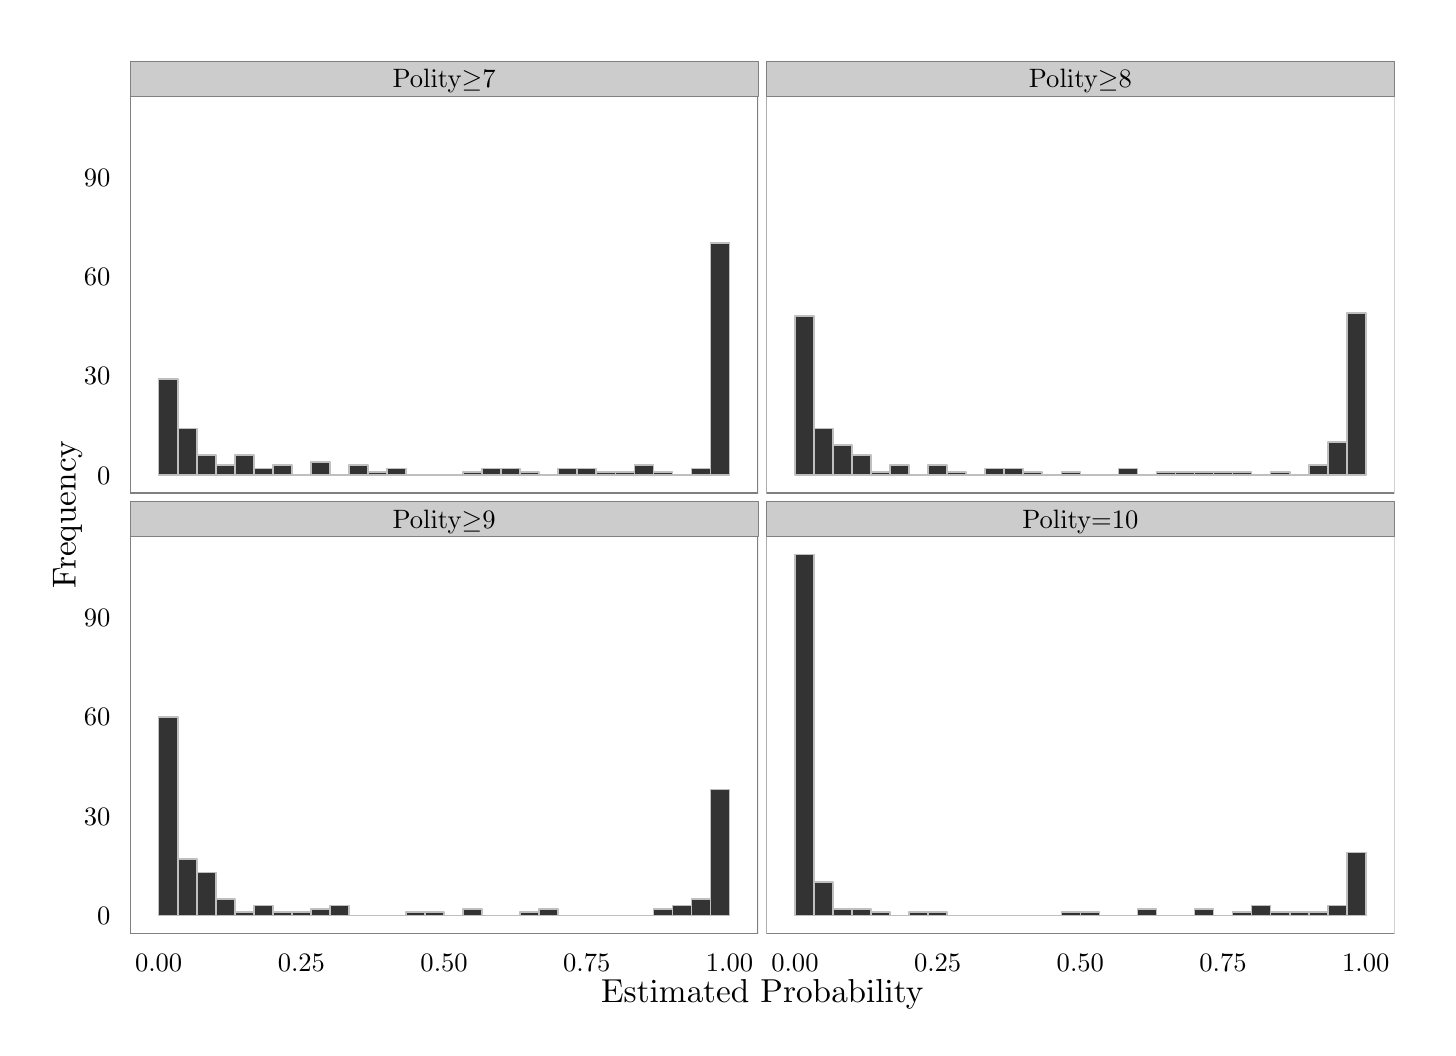
\begin{tikzpicture}[x=1pt,y=1pt]
\definecolor[named]{drawColor}{rgb}{0.00,0.00,0.00}
\definecolor[named]{fillColor}{rgb}{1.00,1.00,1.00}
\fill[color=fillColor,fill opacity=0.00,] (0,0) rectangle (505.89,361.35);
\begin{scope}
\path[clip] (  0.00,  0.00) rectangle (505.89,361.35);
\end{scope}
\begin{scope}
\path[clip] (  0.00,  0.00) rectangle (505.89,361.35);
\end{scope}
\begin{scope}
\path[clip] (  0.00,  0.00) rectangle (505.89,361.35);
\definecolor[named]{drawColor}{rgb}{1.00,1.00,1.00}
\definecolor[named]{fillColor}{rgb}{1.00,1.00,1.00}

\draw[color=drawColor,line width= 0.6pt,line cap=round,line join=round,fill=fillColor,] (  0.00,  0.00) rectangle (505.89,361.35);
\end{scope}
\begin{scope}
\path[clip] (  0.00,  0.00) rectangle (505.89,361.35);
\end{scope}
\begin{scope}
\path[clip] ( 37.02,193.18) rectangle (263.93,336.67);
\definecolor[named]{fillColor}{rgb}{1.00,1.00,1.00}

\draw[fill=fillColor,draw opacity=0.00,] ( 37.02,193.18) rectangle (263.93,336.67);
\definecolor[named]{drawColor}{rgb}{0.75,0.75,0.75}
\definecolor[named]{fillColor}{rgb}{0.20,0.20,0.20}

\draw[color=drawColor,line width= 0.6pt,line join=round,fill=fillColor,] ( 47.33,199.70) rectangle ( 54.21,234.40);

\draw[color=drawColor,line width= 0.6pt,line join=round,fill=fillColor,] ( 54.21,199.70) rectangle ( 61.09,216.45);

\draw[color=drawColor,line width= 0.6pt,line join=round,fill=fillColor,] ( 61.09,199.70) rectangle ( 67.96,206.88);

\draw[color=drawColor,line width= 0.6pt,line join=round,fill=fillColor,] ( 67.96,199.70) rectangle ( 74.84,203.29);

\draw[color=drawColor,line width= 0.6pt,line join=round,fill=fillColor,] ( 74.84,199.70) rectangle ( 81.71,206.88);

\draw[color=drawColor,line width= 0.6pt,line join=round,fill=fillColor,] ( 81.71,199.70) rectangle ( 88.59,202.09);

\draw[color=drawColor,line width= 0.6pt,line join=round,fill=fillColor,] ( 88.59,199.70) rectangle ( 95.47,203.29);

\draw[color=drawColor,line width= 0.6pt,line join=round,fill=fillColor,] ( 95.47,199.70) rectangle (102.34,199.70);

\draw[color=drawColor,line width= 0.6pt,line join=round,fill=fillColor,] (102.34,199.70) rectangle (109.22,204.49);

\draw[color=drawColor,line width= 0.6pt,line join=round,fill=fillColor,] (109.22,199.70) rectangle (116.09,199.70);

\draw[color=drawColor,line width= 0.6pt,line join=round,fill=fillColor,] (116.09,199.70) rectangle (122.97,203.29);

\draw[color=drawColor,line width= 0.6pt,line join=round,fill=fillColor,] (122.97,199.70) rectangle (129.85,200.89);

\draw[color=drawColor,line width= 0.6pt,line join=round,fill=fillColor,] (129.85,199.70) rectangle (136.72,202.09);

\draw[color=drawColor,line width= 0.6pt,line join=round,fill=fillColor,] (136.72,199.70) rectangle (143.60,199.70);

\draw[color=drawColor,line width= 0.6pt,line join=round,fill=fillColor,] (143.60,199.70) rectangle (150.47,199.70);

\draw[color=drawColor,line width= 0.6pt,line join=round,fill=fillColor,] (150.47,199.70) rectangle (157.35,199.70);

\draw[color=drawColor,line width= 0.6pt,line join=round,fill=fillColor,] (157.35,199.70) rectangle (164.23,200.89);

\draw[color=drawColor,line width= 0.6pt,line join=round,fill=fillColor,] (164.23,199.70) rectangle (171.10,202.09);

\draw[color=drawColor,line width= 0.6pt,line join=round,fill=fillColor,] (171.10,199.70) rectangle (177.98,202.09);

\draw[color=drawColor,line width= 0.6pt,line join=round,fill=fillColor,] (177.98,199.70) rectangle (184.85,200.89);

\draw[color=drawColor,line width= 0.6pt,line join=round,fill=fillColor,] (184.85,199.70) rectangle (191.73,199.70);

\draw[color=drawColor,line width= 0.6pt,line join=round,fill=fillColor,] (191.73,199.70) rectangle (198.61,202.09);

\draw[color=drawColor,line width= 0.6pt,line join=round,fill=fillColor,] (198.61,199.70) rectangle (205.48,202.09);

\draw[color=drawColor,line width= 0.6pt,line join=round,fill=fillColor,] (205.48,199.70) rectangle (212.36,200.89);

\draw[color=drawColor,line width= 0.6pt,line join=round,fill=fillColor,] (212.36,199.70) rectangle (219.23,200.89);

\draw[color=drawColor,line width= 0.6pt,line join=round,fill=fillColor,] (219.23,199.70) rectangle (226.11,203.29);

\draw[color=drawColor,line width= 0.6pt,line join=round,fill=fillColor,] (226.11,199.70) rectangle (232.99,200.89);

\draw[color=drawColor,line width= 0.6pt,line join=round,fill=fillColor,] (232.99,199.70) rectangle (239.86,199.70);

\draw[color=drawColor,line width= 0.6pt,line join=round,fill=fillColor,] (239.86,199.70) rectangle (246.74,202.09);

\draw[color=drawColor,line width= 0.6pt,line join=round,fill=fillColor,] (246.74,199.70) rectangle (253.61,283.47);
\definecolor[named]{drawColor}{rgb}{0.50,0.50,0.50}

\draw[color=drawColor,line width= 0.6pt,line cap=round,line join=round,fill opacity=0.00,] ( 37.02,193.18) rectangle (263.93,336.67);
\end{scope}
\begin{scope}
\path[clip] (  0.00,  0.00) rectangle (505.89,361.35);
\end{scope}
\begin{scope}
\path[clip] (266.94,193.18) rectangle (493.85,336.67);
\definecolor[named]{fillColor}{rgb}{1.00,1.00,1.00}

\draw[fill=fillColor,draw opacity=0.00,] (266.94,193.18) rectangle (493.85,336.67);
\definecolor[named]{drawColor}{rgb}{0.75,0.75,0.75}
\definecolor[named]{fillColor}{rgb}{0.20,0.20,0.20}

\draw[color=drawColor,line width= 0.6pt,line join=round,fill=fillColor,] (277.25,199.70) rectangle (284.13,257.14);

\draw[color=drawColor,line width= 0.6pt,line join=round,fill=fillColor,] (284.13,199.70) rectangle (291.00,216.45);

\draw[color=drawColor,line width= 0.6pt,line join=round,fill=fillColor,] (291.00,199.70) rectangle (297.88,210.47);

\draw[color=drawColor,line width= 0.6pt,line join=round,fill=fillColor,] (297.88,199.70) rectangle (304.76,206.88);

\draw[color=drawColor,line width= 0.6pt,line join=round,fill=fillColor,] (304.76,199.70) rectangle (311.63,200.89);

\draw[color=drawColor,line width= 0.6pt,line join=round,fill=fillColor,] (311.63,199.70) rectangle (318.51,203.29);

\draw[color=drawColor,line width= 0.6pt,line join=round,fill=fillColor,] (318.51,199.70) rectangle (325.38,199.70);

\draw[color=drawColor,line width= 0.6pt,line join=round,fill=fillColor,] (325.38,199.70) rectangle (332.26,203.29);

\draw[color=drawColor,line width= 0.6pt,line join=round,fill=fillColor,] (332.26,199.70) rectangle (339.14,200.89);

\draw[color=drawColor,line width= 0.6pt,line join=round,fill=fillColor,] (339.14,199.70) rectangle (346.01,199.70);

\draw[color=drawColor,line width= 0.6pt,line join=round,fill=fillColor,] (346.01,199.70) rectangle (352.89,202.09);

\draw[color=drawColor,line width= 0.6pt,line join=round,fill=fillColor,] (352.89,199.70) rectangle (359.76,202.09);

\draw[color=drawColor,line width= 0.6pt,line join=round,fill=fillColor,] (359.76,199.70) rectangle (366.64,200.89);

\draw[color=drawColor,line width= 0.6pt,line join=round,fill=fillColor,] (366.64,199.70) rectangle (373.52,199.70);

\draw[color=drawColor,line width= 0.6pt,line join=round,fill=fillColor,] (373.52,199.70) rectangle (380.39,200.89);

\draw[color=drawColor,line width= 0.6pt,line join=round,fill=fillColor,] (380.39,199.70) rectangle (387.27,199.70);

\draw[color=drawColor,line width= 0.6pt,line join=round,fill=fillColor,] (387.27,199.70) rectangle (394.14,199.70);

\draw[color=drawColor,line width= 0.6pt,line join=round,fill=fillColor,] (394.14,199.70) rectangle (401.02,202.09);

\draw[color=drawColor,line width= 0.6pt,line join=round,fill=fillColor,] (401.02,199.70) rectangle (407.90,199.70);

\draw[color=drawColor,line width= 0.6pt,line join=round,fill=fillColor,] (407.90,199.70) rectangle (414.77,200.89);

\draw[color=drawColor,line width= 0.6pt,line join=round,fill=fillColor,] (414.77,199.70) rectangle (421.65,200.89);

\draw[color=drawColor,line width= 0.6pt,line join=round,fill=fillColor,] (421.65,199.70) rectangle (428.52,200.89);

\draw[color=drawColor,line width= 0.6pt,line join=round,fill=fillColor,] (428.52,199.70) rectangle (435.40,200.89);

\draw[color=drawColor,line width= 0.6pt,line join=round,fill=fillColor,] (435.40,199.70) rectangle (442.28,200.89);

\draw[color=drawColor,line width= 0.6pt,line join=round,fill=fillColor,] (442.28,199.70) rectangle (449.15,199.70);

\draw[color=drawColor,line width= 0.6pt,line join=round,fill=fillColor,] (449.15,199.70) rectangle (456.03,200.89);

\draw[color=drawColor,line width= 0.6pt,line join=round,fill=fillColor,] (456.03,199.70) rectangle (462.90,199.70);

\draw[color=drawColor,line width= 0.6pt,line join=round,fill=fillColor,] (462.90,199.70) rectangle (469.78,203.29);

\draw[color=drawColor,line width= 0.6pt,line join=round,fill=fillColor,] (469.78,199.70) rectangle (476.66,211.67);

\draw[color=drawColor,line width= 0.6pt,line join=round,fill=fillColor,] (476.66,199.70) rectangle (483.53,258.34);
\definecolor[named]{drawColor}{rgb}{0.50,0.50,0.50}

\draw[color=drawColor,line width= 0.6pt,line cap=round,line join=round,fill opacity=0.00,] (266.94,193.18) rectangle (493.85,336.67);
\end{scope}
\begin{scope}
\path[clip] (  0.00,  0.00) rectangle (505.89,361.35);
\end{scope}
\begin{scope}
\path[clip] ( 37.02, 34.03) rectangle (263.93,177.53);
\definecolor[named]{fillColor}{rgb}{1.00,1.00,1.00}

\draw[fill=fillColor,draw opacity=0.00,] ( 37.02, 34.03) rectangle (263.93,177.53);
\definecolor[named]{drawColor}{rgb}{0.75,0.75,0.75}
\definecolor[named]{fillColor}{rgb}{0.20,0.20,0.20}

\draw[color=drawColor,line width= 0.6pt,line join=round,fill=fillColor,] ( 47.33, 40.56) rectangle ( 54.21,112.36);

\draw[color=drawColor,line width= 0.6pt,line join=round,fill=fillColor,] ( 54.21, 40.56) rectangle ( 61.09, 60.90);

\draw[color=drawColor,line width= 0.6pt,line join=round,fill=fillColor,] ( 61.09, 40.56) rectangle ( 67.96, 56.12);

\draw[color=drawColor,line width= 0.6pt,line join=round,fill=fillColor,] ( 67.96, 40.56) rectangle ( 74.84, 46.54);

\draw[color=drawColor,line width= 0.6pt,line join=round,fill=fillColor,] ( 74.84, 40.56) rectangle ( 81.71, 41.75);

\draw[color=drawColor,line width= 0.6pt,line join=round,fill=fillColor,] ( 81.71, 40.56) rectangle ( 88.59, 44.15);

\draw[color=drawColor,line width= 0.6pt,line join=round,fill=fillColor,] ( 88.59, 40.56) rectangle ( 95.47, 41.75);

\draw[color=drawColor,line width= 0.6pt,line join=round,fill=fillColor,] ( 95.47, 40.56) rectangle (102.34, 41.75);

\draw[color=drawColor,line width= 0.6pt,line join=round,fill=fillColor,] (102.34, 40.56) rectangle (109.22, 42.95);

\draw[color=drawColor,line width= 0.6pt,line join=round,fill=fillColor,] (109.22, 40.56) rectangle (116.09, 44.15);

\draw[color=drawColor,line width= 0.6pt,line join=round,fill=fillColor,] (116.09, 40.56) rectangle (122.97, 40.56);

\draw[color=drawColor,line width= 0.6pt,line join=round,fill=fillColor,] (122.97, 40.56) rectangle (129.85, 40.56);

\draw[color=drawColor,line width= 0.6pt,line join=round,fill=fillColor,] (129.85, 40.56) rectangle (136.72, 40.56);

\draw[color=drawColor,line width= 0.6pt,line join=round,fill=fillColor,] (136.72, 40.56) rectangle (143.60, 41.75);

\draw[color=drawColor,line width= 0.6pt,line join=round,fill=fillColor,] (143.60, 40.56) rectangle (150.47, 41.75);

\draw[color=drawColor,line width= 0.6pt,line join=round,fill=fillColor,] (150.47, 40.56) rectangle (157.35, 40.56);

\draw[color=drawColor,line width= 0.6pt,line join=round,fill=fillColor,] (157.35, 40.56) rectangle (164.23, 42.95);

\draw[color=drawColor,line width= 0.6pt,line join=round,fill=fillColor,] (164.23, 40.56) rectangle (171.10, 40.56);

\draw[color=drawColor,line width= 0.6pt,line join=round,fill=fillColor,] (171.10, 40.56) rectangle (177.98, 40.56);

\draw[color=drawColor,line width= 0.6pt,line join=round,fill=fillColor,] (177.98, 40.56) rectangle (184.85, 41.75);

\draw[color=drawColor,line width= 0.6pt,line join=round,fill=fillColor,] (184.85, 40.56) rectangle (191.73, 42.95);

\draw[color=drawColor,line width= 0.6pt,line join=round,fill=fillColor,] (191.73, 40.56) rectangle (198.61, 40.56);

\draw[color=drawColor,line width= 0.6pt,line join=round,fill=fillColor,] (198.61, 40.56) rectangle (205.48, 40.56);

\draw[color=drawColor,line width= 0.6pt,line join=round,fill=fillColor,] (205.48, 40.56) rectangle (212.36, 40.56);

\draw[color=drawColor,line width= 0.6pt,line join=round,fill=fillColor,] (212.36, 40.56) rectangle (219.23, 40.56);

\draw[color=drawColor,line width= 0.6pt,line join=round,fill=fillColor,] (219.23, 40.56) rectangle (226.11, 40.56);

\draw[color=drawColor,line width= 0.6pt,line join=round,fill=fillColor,] (226.11, 40.56) rectangle (232.99, 42.95);

\draw[color=drawColor,line width= 0.6pt,line join=round,fill=fillColor,] (232.99, 40.56) rectangle (239.86, 44.15);

\draw[color=drawColor,line width= 0.6pt,line join=round,fill=fillColor,] (239.86, 40.56) rectangle (246.74, 46.54);

\draw[color=drawColor,line width= 0.6pt,line join=round,fill=fillColor,] (246.74, 40.56) rectangle (253.61, 86.04);
\definecolor[named]{drawColor}{rgb}{0.50,0.50,0.50}

\draw[color=drawColor,line width= 0.6pt,line cap=round,line join=round,fill opacity=0.00,] ( 37.02, 34.03) rectangle (263.93,177.53);
\end{scope}
\begin{scope}
\path[clip] (  0.00,  0.00) rectangle (505.89,361.35);
\end{scope}
\begin{scope}
\path[clip] (266.94, 34.03) rectangle (493.85,177.53);
\definecolor[named]{fillColor}{rgb}{1.00,1.00,1.00}

\draw[fill=fillColor,draw opacity=0.00,] (266.94, 34.03) rectangle (493.85,177.53);
\definecolor[named]{drawColor}{rgb}{0.75,0.75,0.75}
\definecolor[named]{fillColor}{rgb}{0.20,0.20,0.20}

\draw[color=drawColor,line width= 0.6pt,line join=round,fill=fillColor,] (277.25, 40.56) rectangle (284.13,171.01);

\draw[color=drawColor,line width= 0.6pt,line join=round,fill=fillColor,] (284.13, 40.56) rectangle (291.00, 52.53);

\draw[color=drawColor,line width= 0.6pt,line join=round,fill=fillColor,] (291.00, 40.56) rectangle (297.88, 42.95);

\draw[color=drawColor,line width= 0.6pt,line join=round,fill=fillColor,] (297.88, 40.56) rectangle (304.76, 42.95);

\draw[color=drawColor,line width= 0.6pt,line join=round,fill=fillColor,] (304.76, 40.56) rectangle (311.63, 41.75);

\draw[color=drawColor,line width= 0.6pt,line join=round,fill=fillColor,] (311.63, 40.56) rectangle (318.51, 40.56);

\draw[color=drawColor,line width= 0.6pt,line join=round,fill=fillColor,] (318.51, 40.56) rectangle (325.38, 41.75);

\draw[color=drawColor,line width= 0.6pt,line join=round,fill=fillColor,] (325.38, 40.56) rectangle (332.26, 41.75);

\draw[color=drawColor,line width= 0.6pt,line join=round,fill=fillColor,] (332.26, 40.56) rectangle (339.14, 40.56);

\draw[color=drawColor,line width= 0.6pt,line join=round,fill=fillColor,] (339.14, 40.56) rectangle (346.01, 40.56);

\draw[color=drawColor,line width= 0.6pt,line join=round,fill=fillColor,] (346.01, 40.56) rectangle (352.89, 40.56);

\draw[color=drawColor,line width= 0.6pt,line join=round,fill=fillColor,] (352.89, 40.56) rectangle (359.76, 40.56);

\draw[color=drawColor,line width= 0.6pt,line join=round,fill=fillColor,] (359.76, 40.56) rectangle (366.64, 40.56);

\draw[color=drawColor,line width= 0.6pt,line join=round,fill=fillColor,] (366.64, 40.56) rectangle (373.52, 40.56);

\draw[color=drawColor,line width= 0.6pt,line join=round,fill=fillColor,] (373.52, 40.56) rectangle (380.39, 41.75);

\draw[color=drawColor,line width= 0.6pt,line join=round,fill=fillColor,] (380.39, 40.56) rectangle (387.27, 41.75);

\draw[color=drawColor,line width= 0.6pt,line join=round,fill=fillColor,] (387.27, 40.56) rectangle (394.14, 40.56);

\draw[color=drawColor,line width= 0.6pt,line join=round,fill=fillColor,] (394.14, 40.56) rectangle (401.02, 40.56);

\draw[color=drawColor,line width= 0.6pt,line join=round,fill=fillColor,] (401.02, 40.56) rectangle (407.90, 42.95);

\draw[color=drawColor,line width= 0.6pt,line join=round,fill=fillColor,] (407.90, 40.56) rectangle (414.77, 40.56);

\draw[color=drawColor,line width= 0.6pt,line join=round,fill=fillColor,] (414.77, 40.56) rectangle (421.65, 40.56);

\draw[color=drawColor,line width= 0.6pt,line join=round,fill=fillColor,] (421.65, 40.56) rectangle (428.52, 42.95);

\draw[color=drawColor,line width= 0.6pt,line join=round,fill=fillColor,] (428.52, 40.56) rectangle (435.40, 40.56);

\draw[color=drawColor,line width= 0.6pt,line join=round,fill=fillColor,] (435.40, 40.56) rectangle (442.28, 41.75);

\draw[color=drawColor,line width= 0.6pt,line join=round,fill=fillColor,] (442.28, 40.56) rectangle (449.15, 44.15);

\draw[color=drawColor,line width= 0.6pt,line join=round,fill=fillColor,] (449.15, 40.56) rectangle (456.03, 41.75);

\draw[color=drawColor,line width= 0.6pt,line join=round,fill=fillColor,] (456.03, 40.56) rectangle (462.90, 41.75);

\draw[color=drawColor,line width= 0.6pt,line join=round,fill=fillColor,] (462.90, 40.56) rectangle (469.78, 41.75);

\draw[color=drawColor,line width= 0.6pt,line join=round,fill=fillColor,] (469.78, 40.56) rectangle (476.66, 44.15);

\draw[color=drawColor,line width= 0.6pt,line join=round,fill=fillColor,] (476.66, 40.56) rectangle (483.53, 63.30);
\definecolor[named]{drawColor}{rgb}{0.50,0.50,0.50}

\draw[color=drawColor,line width= 0.6pt,line cap=round,line join=round,fill opacity=0.00,] (266.94, 34.03) rectangle (493.85,177.53);
\end{scope}
\begin{scope}
\path[clip] (  0.00,  0.00) rectangle (505.89,361.35);
\end{scope}
\begin{scope}
\path[clip] (  0.00,  0.00) rectangle (505.89,361.35);
\definecolor[named]{drawColor}{rgb}{0.50,0.50,0.50}
\definecolor[named]{fillColor}{rgb}{0.80,0.80,0.80}

\draw[color=drawColor,line width= 0.2pt,line cap=round,line join=round,fill=fillColor,] ( 37.02,336.67) rectangle (263.93,349.31);
\definecolor[named]{drawColor}{rgb}{0.00,0.00,0.00}

\node[color=drawColor,anchor=base,inner sep=0pt, outer sep=0pt, scale=  0.96] at (150.47,339.68) {Polity$\geq$7};
\end{scope}
\begin{scope}
\path[clip] (  0.00,  0.00) rectangle (505.89,361.35);
\end{scope}
\begin{scope}
\path[clip] (  0.00,  0.00) rectangle (505.89,361.35);
\definecolor[named]{drawColor}{rgb}{0.50,0.50,0.50}
\definecolor[named]{fillColor}{rgb}{0.80,0.80,0.80}

\draw[color=drawColor,line width= 0.2pt,line cap=round,line join=round,fill=fillColor,] (266.94,336.67) rectangle (493.85,349.31);
\definecolor[named]{drawColor}{rgb}{0.00,0.00,0.00}

\node[color=drawColor,anchor=base,inner sep=0pt, outer sep=0pt, scale=  0.96] at (380.39,339.68) {Polity$\geq$8};
\end{scope}
\begin{scope}
\path[clip] (  0.00,  0.00) rectangle (505.89,361.35);
\end{scope}
\begin{scope}
\path[clip] (  0.00,  0.00) rectangle (505.89,361.35);
\definecolor[named]{drawColor}{rgb}{0.50,0.50,0.50}
\definecolor[named]{fillColor}{rgb}{0.80,0.80,0.80}

\draw[color=drawColor,line width= 0.2pt,line cap=round,line join=round,fill=fillColor,] ( 37.02,177.53) rectangle (263.93,190.16);
\definecolor[named]{drawColor}{rgb}{0.00,0.00,0.00}

\node[color=drawColor,anchor=base,inner sep=0pt, outer sep=0pt, scale=  0.96] at (150.47,180.54) {Polity$\geq$9};
\end{scope}
\begin{scope}
\path[clip] (  0.00,  0.00) rectangle (505.89,361.35);
\end{scope}
\begin{scope}
\path[clip] (  0.00,  0.00) rectangle (505.89,361.35);
\definecolor[named]{drawColor}{rgb}{0.50,0.50,0.50}
\definecolor[named]{fillColor}{rgb}{0.80,0.80,0.80}

\draw[color=drawColor,line width= 0.2pt,line cap=round,line join=round,fill=fillColor,] (266.94,177.53) rectangle (493.85,190.16);
\definecolor[named]{drawColor}{rgb}{0.00,0.00,0.00}

\node[color=drawColor,anchor=base,inner sep=0pt, outer sep=0pt, scale=  0.96] at (380.39,180.54) {Polity$=$10};
\end{scope}
\begin{scope}
\path[clip] (  0.00,  0.00) rectangle (505.89,361.35);
\end{scope}
\begin{scope}
\path[clip] (  0.00,  0.00) rectangle (505.89,361.35);
\end{scope}
\begin{scope}
\path[clip] (  0.00,  0.00) rectangle (505.89,361.35);
\definecolor[named]{drawColor}{rgb}{0.00,0.00,0.00}

\node[color=drawColor,anchor=base east,inner sep=0pt, outer sep=0pt, scale=  0.96] at ( 29.91,196.39) {0};

\node[color=drawColor,anchor=base east,inner sep=0pt, outer sep=0pt, scale=  0.96] at ( 29.91,232.30) {30};

\node[color=drawColor,anchor=base east,inner sep=0pt, outer sep=0pt, scale=  0.96] at ( 29.91,268.20) {60};

\node[color=drawColor,anchor=base east,inner sep=0pt, outer sep=0pt, scale=  0.96] at ( 29.91,304.10) {90};
\end{scope}
\begin{scope}
\path[clip] (  0.00,  0.00) rectangle (505.89,361.35);
\end{scope}
\begin{scope}
\path[clip] (  0.00,  0.00) rectangle (505.89,361.35);
\end{scope}
\begin{scope}
\path[clip] (  0.00,  0.00) rectangle (505.89,361.35);
\end{scope}
\begin{scope}
\path[clip] (  0.00,  0.00) rectangle (505.89,361.35);
\end{scope}
\begin{scope}
\path[clip] (  0.00,  0.00) rectangle (505.89,361.35);
\end{scope}
\begin{scope}
\path[clip] (  0.00,  0.00) rectangle (505.89,361.35);
\end{scope}
\begin{scope}
\path[clip] (  0.00,  0.00) rectangle (505.89,361.35);
\end{scope}
\begin{scope}
\path[clip] (  0.00,  0.00) rectangle (505.89,361.35);
\end{scope}
\begin{scope}
\path[clip] (  0.00,  0.00) rectangle (505.89,361.35);
\end{scope}
\begin{scope}
\path[clip] (  0.00,  0.00) rectangle (505.89,361.35);
\definecolor[named]{drawColor}{rgb}{0.00,0.00,0.00}

\node[color=drawColor,anchor=base east,inner sep=0pt, outer sep=0pt, scale=  0.96] at ( 29.91, 37.25) {0};

\node[color=drawColor,anchor=base east,inner sep=0pt, outer sep=0pt, scale=  0.96] at ( 29.91, 73.15) {30};

\node[color=drawColor,anchor=base east,inner sep=0pt, outer sep=0pt, scale=  0.96] at ( 29.91,109.06) {60};

\node[color=drawColor,anchor=base east,inner sep=0pt, outer sep=0pt, scale=  0.96] at ( 29.91,144.96) {90};
\end{scope}
\begin{scope}
\path[clip] (  0.00,  0.00) rectangle (505.89,361.35);
\end{scope}
\begin{scope}
\path[clip] (  0.00,  0.00) rectangle (505.89,361.35);
\end{scope}
\begin{scope}
\path[clip] (  0.00,  0.00) rectangle (505.89,361.35);
\end{scope}
\begin{scope}
\path[clip] (  0.00,  0.00) rectangle (505.89,361.35);
\end{scope}
\begin{scope}
\path[clip] (  0.00,  0.00) rectangle (505.89,361.35);
\end{scope}
\begin{scope}
\path[clip] (  0.00,  0.00) rectangle (505.89,361.35);
\end{scope}
\begin{scope}
\path[clip] (  0.00,  0.00) rectangle (505.89,361.35);
\end{scope}
\begin{scope}
\path[clip] (  0.00,  0.00) rectangle (505.89,361.35);
\end{scope}
\begin{scope}
\path[clip] (  0.00,  0.00) rectangle (505.89,361.35);
\end{scope}
\begin{scope}
\path[clip] (  0.00,  0.00) rectangle (505.89,361.35);
\end{scope}
\begin{scope}
\path[clip] (  0.00,  0.00) rectangle (505.89,361.35);
\end{scope}
\begin{scope}
\path[clip] (  0.00,  0.00) rectangle (505.89,361.35);
\end{scope}
\begin{scope}
\path[clip] (  0.00,  0.00) rectangle (505.89,361.35);
\end{scope}
\begin{scope}
\path[clip] (  0.00,  0.00) rectangle (505.89,361.35);
\end{scope}
\begin{scope}
\path[clip] (  0.00,  0.00) rectangle (505.89,361.35);
\end{scope}
\begin{scope}
\path[clip] (  0.00,  0.00) rectangle (505.89,361.35);
\definecolor[named]{drawColor}{rgb}{0.00,0.00,0.00}

\node[color=drawColor,anchor=base,inner sep=0pt, outer sep=0pt, scale=  0.96] at ( 47.33, 20.31) {0.00};

\node[color=drawColor,anchor=base,inner sep=0pt, outer sep=0pt, scale=  0.96] at ( 98.90, 20.31) {0.25};

\node[color=drawColor,anchor=base,inner sep=0pt, outer sep=0pt, scale=  0.96] at (150.47, 20.31) {0.50};

\node[color=drawColor,anchor=base,inner sep=0pt, outer sep=0pt, scale=  0.96] at (202.04, 20.31) {0.75};

\node[color=drawColor,anchor=base,inner sep=0pt, outer sep=0pt, scale=  0.96] at (253.61, 20.31) {1.00};
\end{scope}
\begin{scope}
\path[clip] (  0.00,  0.00) rectangle (505.89,361.35);
\end{scope}
\begin{scope}
\path[clip] (  0.00,  0.00) rectangle (505.89,361.35);
\end{scope}
\begin{scope}
\path[clip] (  0.00,  0.00) rectangle (505.89,361.35);
\end{scope}
\begin{scope}
\path[clip] (  0.00,  0.00) rectangle (505.89,361.35);
\end{scope}
\begin{scope}
\path[clip] (  0.00,  0.00) rectangle (505.89,361.35);
\end{scope}
\begin{scope}
\path[clip] (  0.00,  0.00) rectangle (505.89,361.35);
\end{scope}
\begin{scope}
\path[clip] (  0.00,  0.00) rectangle (505.89,361.35);
\end{scope}
\begin{scope}
\path[clip] (  0.00,  0.00) rectangle (505.89,361.35);
\definecolor[named]{drawColor}{rgb}{0.00,0.00,0.00}

\node[color=drawColor,anchor=base,inner sep=0pt, outer sep=0pt, scale=  0.96] at (277.25, 20.31) {0.00};

\node[color=drawColor,anchor=base,inner sep=0pt, outer sep=0pt, scale=  0.96] at (328.82, 20.31) {0.25};

\node[color=drawColor,anchor=base,inner sep=0pt, outer sep=0pt, scale=  0.96] at (380.39, 20.31) {0.50};

\node[color=drawColor,anchor=base,inner sep=0pt, outer sep=0pt, scale=  0.96] at (431.96, 20.31) {0.75};

\node[color=drawColor,anchor=base,inner sep=0pt, outer sep=0pt, scale=  0.96] at (483.53, 20.31) {1.00};
\end{scope}
\begin{scope}
\path[clip] (  0.00,  0.00) rectangle (505.89,361.35);
\end{scope}
\begin{scope}
\path[clip] (  0.00,  0.00) rectangle (505.89,361.35);
\end{scope}
\begin{scope}
\path[clip] (  0.00,  0.00) rectangle (505.89,361.35);
\end{scope}
\begin{scope}
\path[clip] (  0.00,  0.00) rectangle (505.89,361.35);
\end{scope}
\begin{scope}
\path[clip] (  0.00,  0.00) rectangle (505.89,361.35);
\definecolor[named]{drawColor}{rgb}{0.00,0.00,0.00}

\node[color=drawColor,anchor=base,inner sep=0pt, outer sep=0pt, scale=  1.20] at (265.43,  9.03) {Estimated Probability};
\end{scope}
\begin{scope}
\path[clip] (  0.00,  0.00) rectangle (505.89,361.35);
\end{scope}
\begin{scope}
\path[clip] (  0.00,  0.00) rectangle (505.89,361.35);
\definecolor[named]{drawColor}{rgb}{0.00,0.00,0.00}

\node[rotate= 90.00,color=drawColor,anchor=base,inner sep=0pt, outer sep=0pt, scale=  1.20] at ( 17.30,185.35) {Frequency};
\end{scope}
\begin{scope}
\path[clip] (  0.00,  0.00) rectangle (505.89,361.35);
\end{scope}
\begin{scope}
\path[clip] (  0.00,  0.00) rectangle (505.89,361.35);
\end{scope}
\begin{scope}
\path[clip] (  0.00,  0.00) rectangle (505.89,361.35);
\end{scope}
\begin{scope}
\path[clip] (  0.00,  0.00) rectangle (505.89,361.35);
\end{scope}
\end{tikzpicture}
